\chapter{Interfaccia}
  \label{chapter_interfaccia}
  All'interno di questo capitolo vengono mostrate le interfacce sviluppate per la web application e descritte le funzionalità
  che sono state implementate. Le funzionalità descritte sono quelle relative all'utente amministratore, che ha accesso a tutte
  le funzionalità della web application.
  \section{Login}
  La schermata \textit{Login}, visibile nella \textit{Figura \ref{fig:Login}}, permette di visualizzare un form per
  l'inserimento delle credenziali d'accesso alla web application. Le credenziali richieste sono username e password e
  sono legate alle credenziali di dominio dell'utente che deve effettuare il login. La verifica delle credenziali viene
  effettuata lato server, confrontando le credenziali inserite con quelle di dominio. Una volta che le credenziali vengono
  verificate e sono corrette, viene verificata la presenza dell'utente nel database, per ricavare le informazioni sulle
  funzionalità alle quali può accedere l'utente loggato in base al gruppo di appartenenza.
  \begin{figure}[H]
    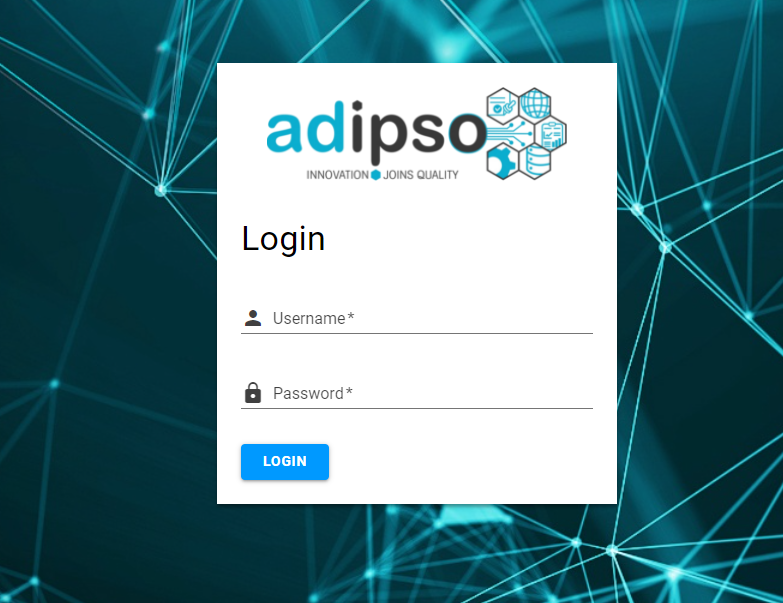
\includegraphics[width=0.75\textwidth]{Login}
    \centering
    \caption{\textit{Schermata di Login}}
    \label{fig:Login}
  \end{figure}

  \section{Storico Colate}
  La schermata \textit{Storico Colate}, visibile nella \textit{Figura \ref{fig:StoricoColate}}, permette di visualizzare
  l'elenco delle colate che sono state schedulate. La pagina contiene un filtro temporale che consente di filtrare
  le colate visualizzate in base ai filtri impostati. La pagina è divisa in due sezioni orizzontali. La prima sezione
  mostra le informazioni relative alle colate base,
  come le date di inizio e di fine previste e effettive, lo stato e l'operatore che ha effettuato operazioni sulla colata.
  Selezionando una colata vengono mostrati due pulsanti. Uno consente di visualizzare il popup visibile 
  nella \textit{Figura \ref{fig:ViewDetailLeghe}},
  che mostra i dettagli relativi alla lega collegata alla colata selezionata come il relativo cliente, nome e descrizione. 
  L'altro pulsante invece consente di aggiungere un nuovo output relativo alla colata selezionata tramite un popup. 
  Questo popup consente di inserire i dati relativi a un nuovo inserimento di un output relativo alla
  colata selezionata. I dati in questione sono la data di scorifica, il tipo di output, il cassone in cui si trova l'output,
  la qualità dell'output e eventuali note.\\
  Con la selezione di una colata base viene anche popolata la seconda sezione con le informazioni relative alle colate specifiche
  che sono collegate alla colata base selezionata. Anche per quanto riguarda le colate specifiche, selezionando 
  una colata vengono abilitati due pulsanti analoghi a quelli descritti per le colate base.
  
  \begin{figure}[H]
    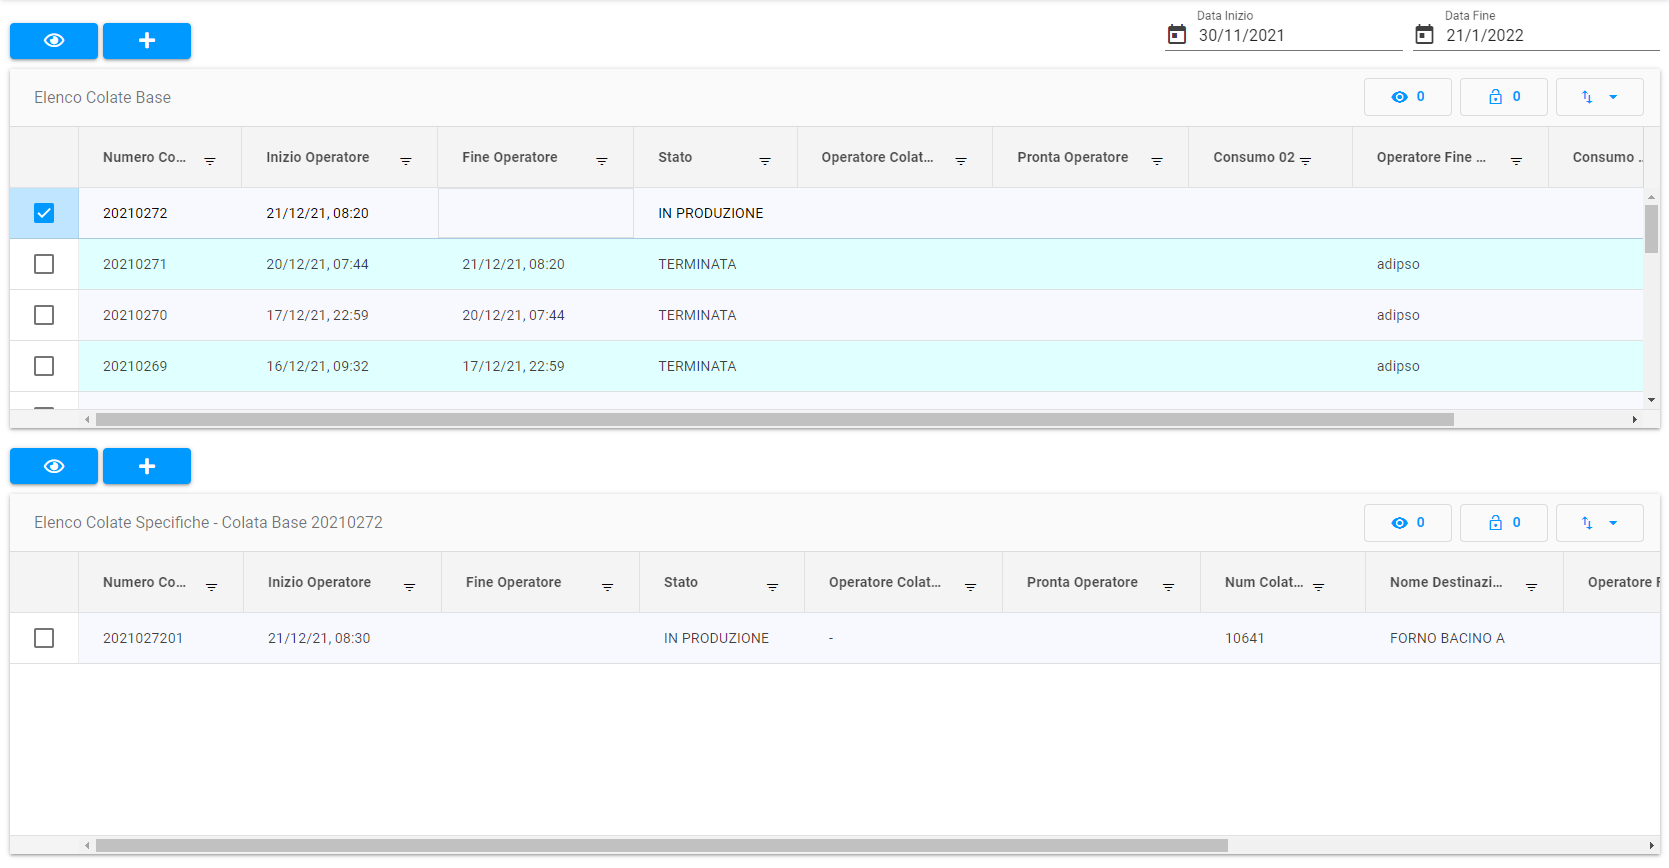
\includegraphics[width = \columnwidth]{StoricoColate}
    \centering
    \caption{\textit{Schermata Storico Colate}}
    \label{fig:StoricoColate}
  \end{figure}

  \begin{figure}[H]
    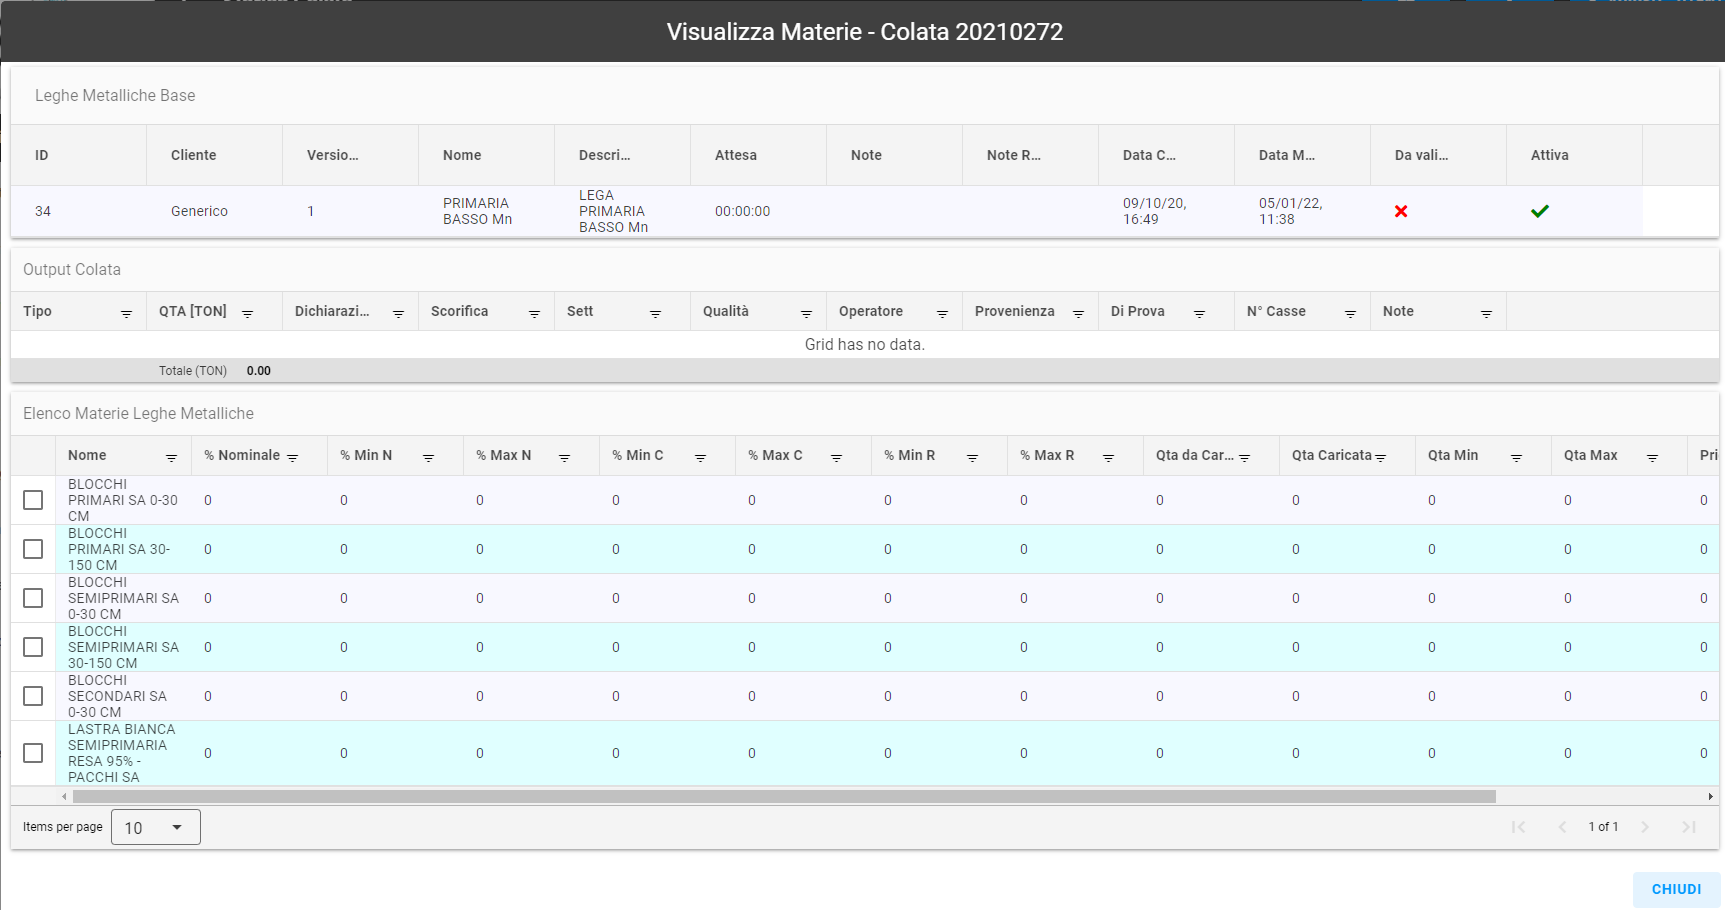
\includegraphics[width = \columnwidth]{ViewDetailLeghe}
    \centering
    \caption{\textit{Popup Dettagli Lega}}
    \label{fig:ViewDetailLeghe}
  \end{figure}
  
  \section{Schede Colaticci}
  La schermata \textit{Schede Colaticci} permette di visualizzare l'elenco delle schede colaticci
  attualmente aperte e quelle chiuse. La pagina contiene un filtro che consente di filtrare le schede tra aperte e chiuse ed
  è divisa in due sezioni orizzontali. Le due sezioni mostrano rispettivamente le informazioni sulle schede base e sulle schede
  specifiche.\\
  Nella pagina relativa alle schede aperte, visibile nella \textit{Figura \ref{fig:SchedeColaticciAperte}}, vengono
  visualizzate le relative informazioni come il numero di scheda, la data di apertura della scheda e la quantità totale
  degli output contenuti nella scheda. Nella pagina è presente un pulsante che consente di inserire una nuova scheda manualmente. 

  \begin{figure}[H]
    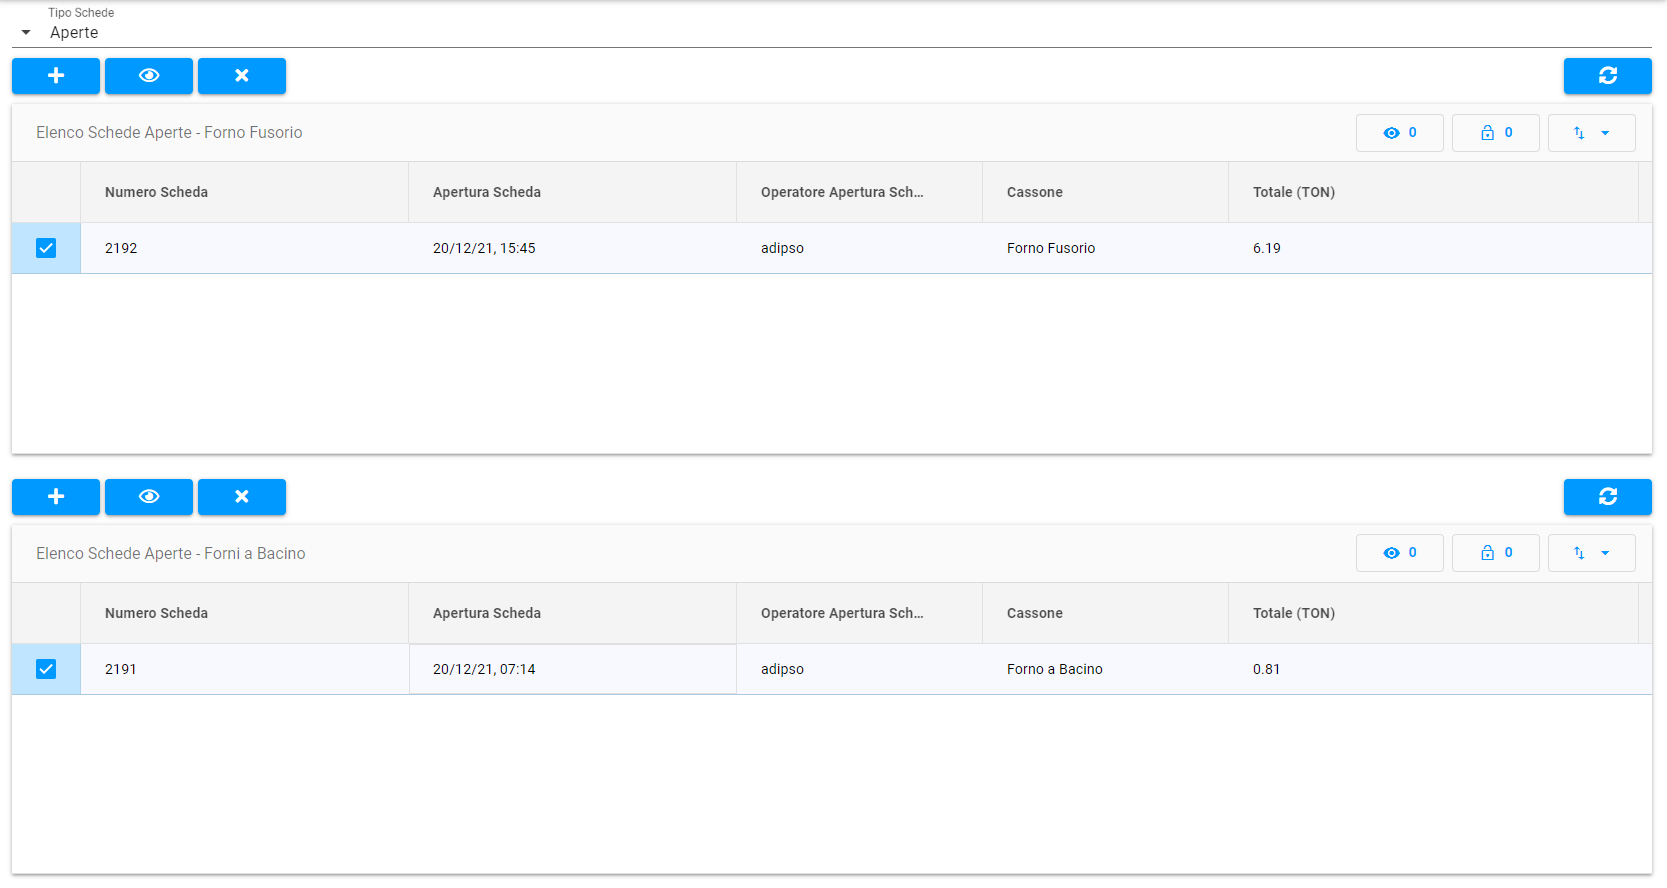
\includegraphics[width = \columnwidth]{SchedeColaticciAperte}
    \centering
    \caption{\textit{Schermata Schede Colaticci Aperte}}
    \label{fig:SchedeColaticciAperte}
  \end{figure}
    
  Inoltre, se viene selezionata una scheda vengono mostrati altri due pulsanti. Il primo pulsante apre
  il popup visibile nella \textit{Figura \ref{fig:DettaglioSchedaColaticci}}, che consente di visualizzare i dettagli 
  della scheda, ovvero tutte le informazioni degli output relativi alla scheda selezionata, come la quantità, 
  l'operatore che ha inserito l'output, la data di dicharazione e la qualità. In questo popup inoltre è possibile
  aggiungere un nuovo output, modificarne uno già inserito, spostare un output in un altra scheda o chiudere la
  scheda selezionata. Il secondo pulsante invece chiude la scheda selezionata. Una volta che una scheda viene chiusa ne viene
  aperta una nuova automaticamente per lo stesso cassone di quella che è appena stata chiusa.\\
  
  \begin{figure}[H]
    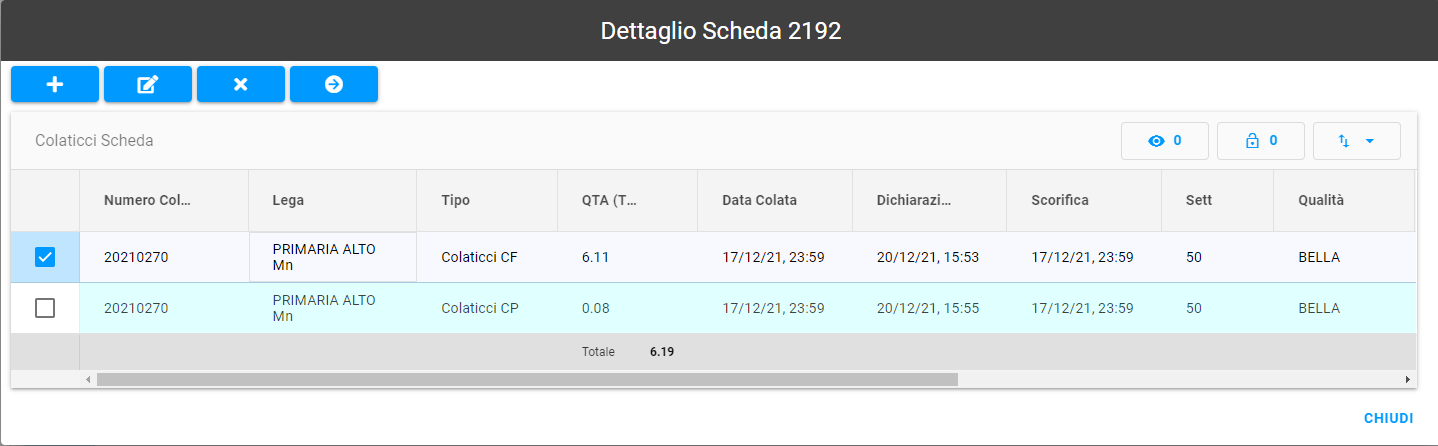
\includegraphics[width = \columnwidth]{DettaglioSchedaColaticci}
    \centering
    \caption{\textit{Popup Dettagli Scheda Colaticci}}
    \label{fig:DettaglioSchedaColaticci}
  \end{figure}
  
  Invece, nella pagina relativa alle schede chiuse, visibile nella \textit{Figura \ref{fig:SchedeColaticciChiuse}}
  vengono visualizzate le relative informazioni come il numero di scheda,
  il relativo stato, il progressivo del camion utilizzato per la spedizione della scheda, il numero di DDT e le date di apertura,
  chiusura e spedizione della scheda. Selezionando una scheda è possibile visualizzarne i dettagli tramite un popup analogo a
  quello descritto in precedenza, nel quale vengono visualizzati i dettagli degli output relativi alla scheda selezionata.
  Inoltre se viene selezionata una scheda non spedita, è possibile inserire i dati di spedizione, come il numero del camion
  e il numero del DDT e dichiarare la scheda come spedita.

  \begin{figure}[H]
    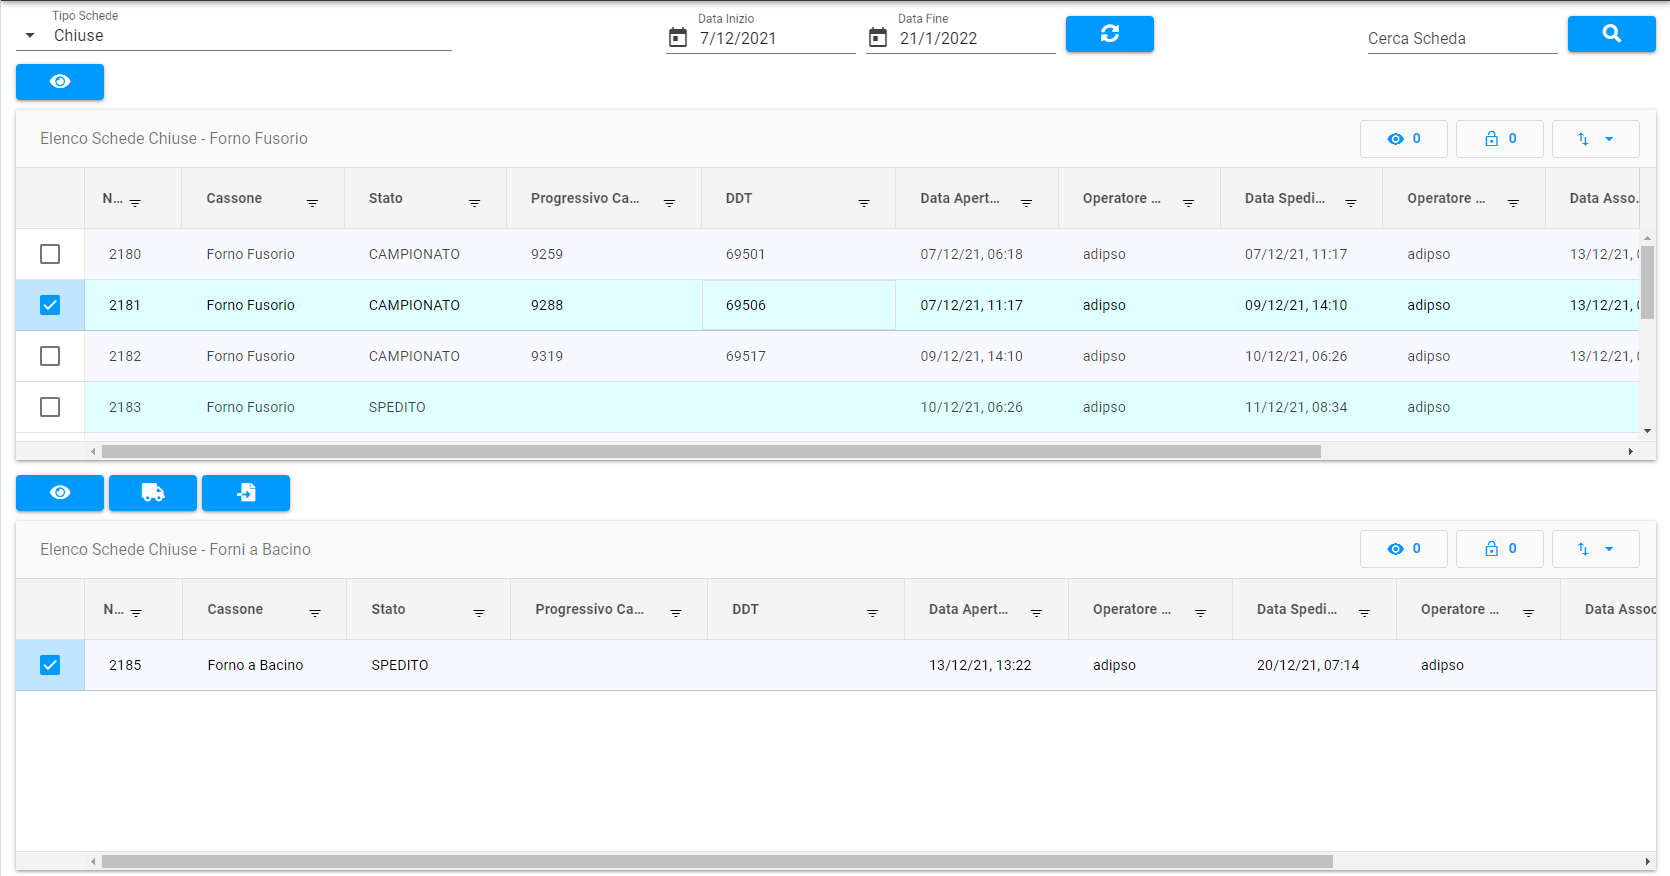
\includegraphics[width = \columnwidth]{SchedeColaticciChiuse}
    \centering
    \caption{\textit{Schermata Schede Colaticci Chiuse}}
    \label{fig:SchedeColaticciChiuse}
  \end{figure}
  

  
  \section{Rapporti Di Lavoro Forno Fusorio}
  La schermata \textit{Rapporti Di Lavoro Forno Fusorio} permette di visualizzare
  i rapporti di lavoro relativi all'impianto del Forno Fusorio. Le informazioni visualizzate vengono filtrate in base al turno.
  Di default vengono mostrate le informazioni relative al turno attuale e quello precedente, anche se la data di inizio è
  modificabile. Nella schermata vengono visualizzate le informazioni sul turno e sulla colata attuali, oltre che all'operatore
  di supporto per il turno in corso. Inoltre sono visibili le seguenti tabelle che mostrano informazioni relative al 
  rapporto di lavoro:
  \begin{itemize}
    \item \textit{Carichi Materiale}. Questa tabella contiene l'elenco dei materiali schedulati che devono essere caricati nella
    colata attualmente in corso e eventuali materiali non pianificati. In questa tabella vengono visualizzati i vari materiali
    con la relativa quantità da caricare, la quantità già caricata, il numero della carica in corso e il dettaglio dei
    carichi effettuati per ogni materiale. Inoltre è possibile aggiungere nuovi carichi o nuovi materiali non pianificati e
    eliminare un carico inserito in precedenza. La tabella è visibile nella \textit{Figura \ref{fig:CarichiMaterialiFfu}};

    \begin{figure}[H]
      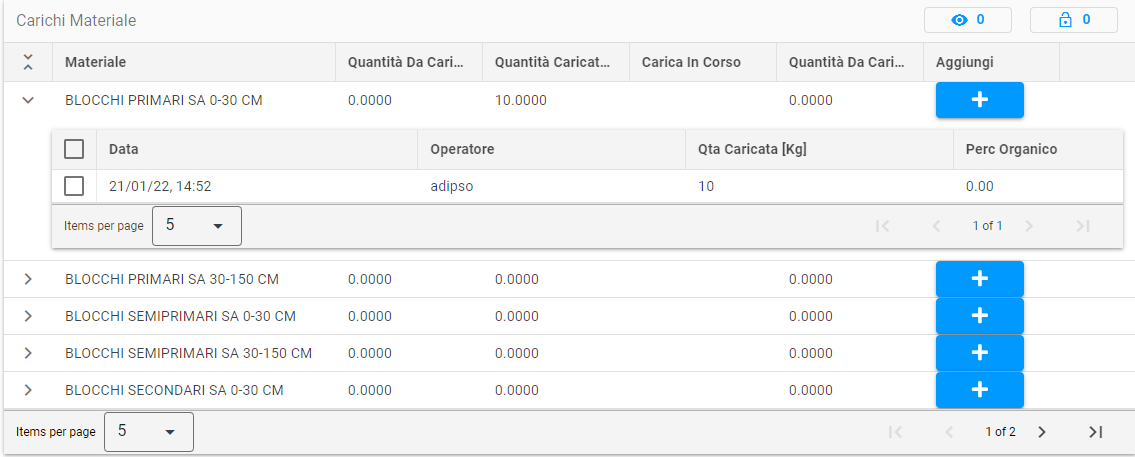
\includegraphics[width = \columnwidth]{CarichiMaterialiFfu}
      \centering
      \caption{\textit{Carichi Materiali Forno Fusorio}}
      \label{fig:CarichiMaterialiFfu}
    \end{figure}

    \item \textit{Piano Cariche}. Questa tabella contiene l'elenco delle cariche che sono state pianificate nel range temporale
    selezionato tramite i filtri. Le informazioni contenute in questa tabella sono il numero della carica e, per
    ogni materiale, la quantità prevista. La tabella è visibile nella \textit{Figura \ref{fig:PianoCaricheFfu}};

    \begin{figure}[H]
      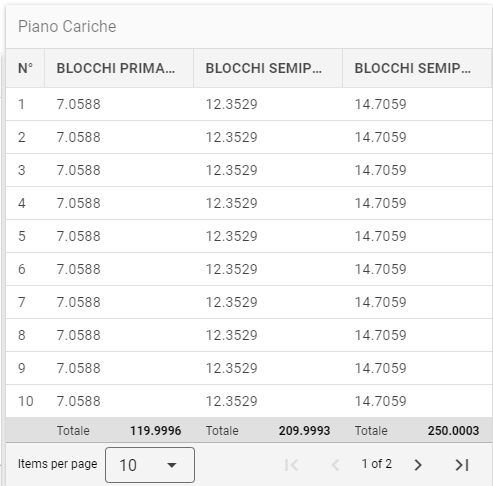
\includegraphics[width=0.5\textwidth]{PianoCaricheFfu}
      \centering
      \caption{\textit{Piano Cariche Forno Fusorio}}
      \label{fig:PianoCaricheFfu}
    \end{figure}


    \item \textit{Output Colata}. Questa tabella contiene le informazioni relative agli output relativi alla colata in corso
    e rilevati nel range temporale selezionato tramite i filtri. Le informazioni visualizzate sono la quantità,
    la data di dichiarazione, la qualità, l'operatore che ha inserito l'output e eventuali note. Inoltre è possibile
    inserire un nuovo output colata. La tabella è visibile nella \textit{Figura \ref{fig:OutputColata}};

    \begin{figure}[H]
      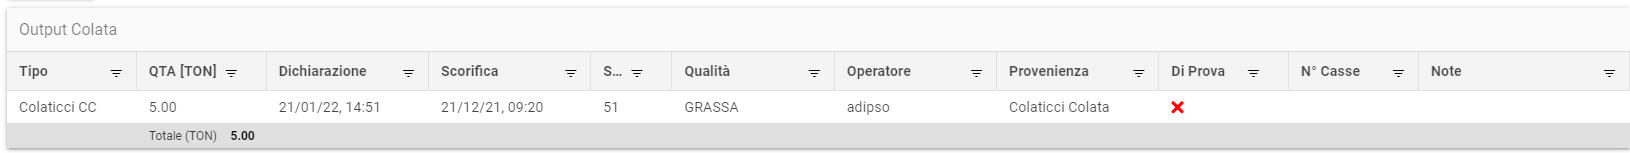
\includegraphics[width = \columnwidth]{OutputColata}
      \centering
      \caption{\textit{Elenco Output Colata}}
      \label{fig:OutputColata}
    \end{figure}

    \item \textit{Elenco Fermi}. Questa tabella contiene l'elenco dei fermi rilevati nel range temporale selezionato tramite i
    filtri e quelli ancora non causalizzati. I fermi sono filtrabili tra quelli causalizzati e quelli non causalizzati,
    che hanno lo sfondo arancione, per differenziarli da quelli causalizzati. Le informazioni visualizzate sono la data
    e l'ora di inizio e di fine del fermo, la durata totale, i cinque perchè e l'azione correttiva. Inoltre è possibile
    causalizzare i fermi non causalizzati e aggiungere nuovi fermi manualmente. La tabella è visibile nella 
    \textit{Figura \ref{fig:ElencoFermi}};
    
    \begin{figure}[H]
      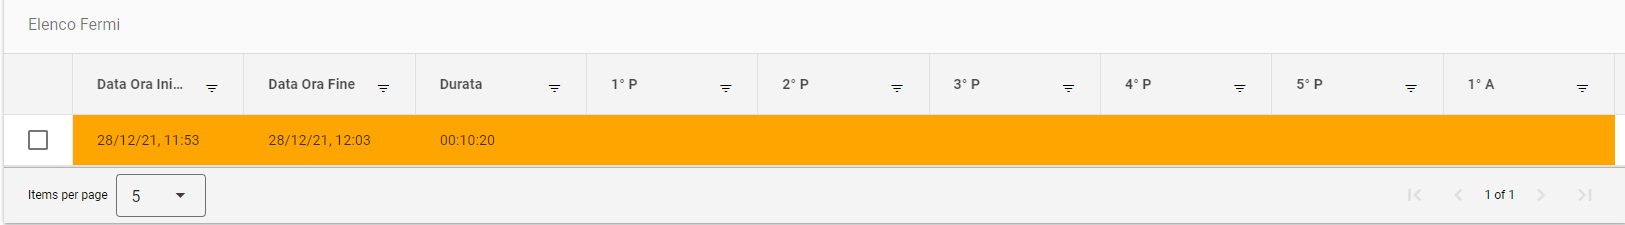
\includegraphics[width = \columnwidth]{ElencoFermi}
      \centering
      \caption{\textit{Elenco Fermi}}
      \label{fig:ElencoFermi}
    \end{figure}
    
    
    \item \textit{Elenco Anomalie}. Questa tabella contiene l'elenco delle anomalie che sono state rilevate  nel range
    temporale selezionato tramite i filtri. Le informazioni visualizzate in questa tabella sono la data di rilevazione
    dell'anomalia, l'operatore che ha inserito l'anomalia, il tipo e la descrizione. Inoltre è possibile anche aggiungere
    una nuova anomalia. La tabella è visibile nella \textit{Figura \ref{fig:ElencoAnomalie}};

    \begin{figure}[H]
      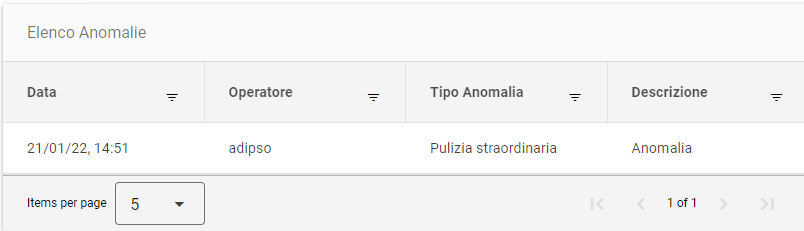
\includegraphics[width = \columnwidth]{ElencoAnomalie}
      \centering
      \caption{\textit{Elenco Anomalie}}
      \label{fig:ElencoAnomalie}
    \end{figure}

    \item \textit{Elenco Note Turno Corrente}. Questa tabella contiene l'elenco delle note che sono state inserite nel corso
    del turno attuale. Le informazioni visualizzate in questa tabella sono la data di inserimento, l'operatore che ha inserito
    la nota e la nota stessa. Inoltre è possibile aggiungere nuove note. La tabella è visibile nella 
    \textit{Figura \ref{fig:ElencoNote}};

    \begin{figure}[H]
      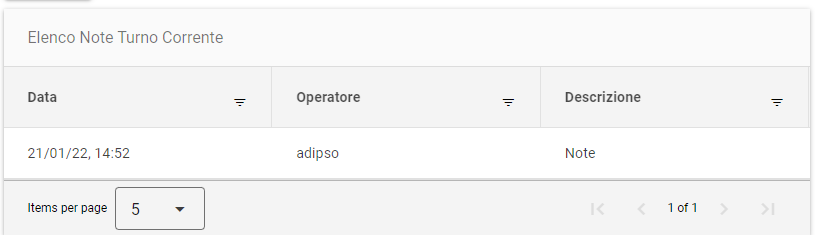
\includegraphics[width = \columnwidth]{ElencoNote}
      \centering
      \caption{\textit{Elenco Note}}
      \label{fig:ElencoNote}
    \end{figure}

    \item \textit{Elenco Note Turno Precedente}. Questa tabella contiene l'elenco delle note che sono state inserite in
    un range temporale che va dalla data di inizio selezionata e la fine del turno precedente. Le informazioni visualizzate sono
    le stesse visualizzate nella tabella contenente le note relative al turno corrente.
  \end{itemize}

  \section{Rapporti Di Lavoro Forni a Bacino}
  La schermata \textit{Rapporti Di Lavoro Forni a Bacino} permette di visualizzare
  i rapporti di lavoro relativi agli impianti dei Forni a Bacino. Le informazioni visualizzate vengono filtrate in base al
  forno a bacino e alla colata selezionati. Di default vengono mostrate le informazioni relative alla colata in corso.
  Nella schermata vengono visualizzate le informazioni sul turno attuale e sulla colata selezionata, oltre che all'operatore
  di supporto per il turno in corso. Inoltre sono visibili le seguenti tabelle che mostrano informazioni relative al 
  rapporto di lavoro:
  \begin{itemize}
    \item \textit{Carichi Materiale}. Questa tabella contiene l'elenco dei materiali schedulati che devono essere caricati nella
    colata attualmente in corso e eventuali materiali non pianificati. In questa tabella vengono visualizzati i vari materiali
    con la relativa quantità da caricare, la quantità già caricata, lo stato della carica e il dettaglio dei carichi effettuati
    per ogni materiale. Inoltre è possibile aggiungere nuovi carichi o nuovi materiali non pianificati, eliminare un carico
    inserito in precedenza e infine chiudere la carica di un determinato materiale. La tabella è visibile nella
    \textit{Figura \ref{fig:CarichiMaterialiFb}};

    \begin{figure}[H]
      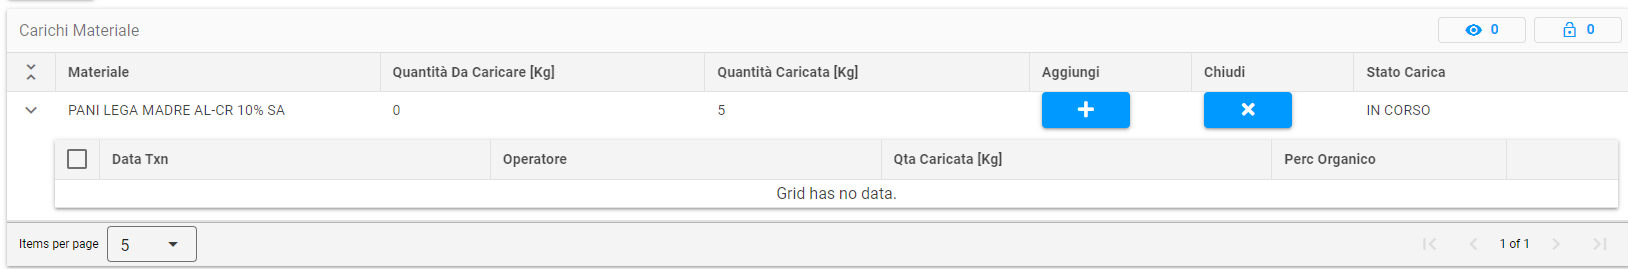
\includegraphics[width = \columnwidth]{CarichiMaterialiFb}
      \centering
      \caption{\textit{Carichi Materiali Forno a Bacino}}
      \label{fig:CarichiMaterialiFb}
    \end{figure}

    \item \textit{Output Colata}. Questa tabella contiene le informazioni relative agli output relativi alla colata selezionata.
    Le informazioni visualizzate sono la quantità, la data di dichiarazione, la qualità, l'operatore che ha inserito l'output
    e eventuali note. Inoltre è possibile inserire un nuovo output colata per la colata selezionata. La tabella è visibile 
    nella \textit{Figura \ref{fig:OutputColata}};

    \item \textit{Elenco Anomalie}. Questa tabella contiene l'elenco delle anomalie che sono state rilevate durante la colata
    selezionata. Le informazioni visualizzate in questa tabella sono la data di rilevazione dell'anomalia, l'operatore che
    ha inserito l'anomalia, il tipo e la descrizione. Inoltre è possibile anche aggiungere una nuova anomalia per la
    colata selezionata. La tabella è visibile nella \textit{Figura \ref{fig:ElencoAnomalie}};

    \item \textit{Elenco Note Turno Corrente}. Questa tabella contiene l'elenco delle note che sono state inserite nel corso
    del turno corrente. Le informazioni visualizzate in questa tabella sono la data di inserimento, l'operatore che ha inserito
    la nota e la nota stessa. Inoltre è possibile aggiungere nuove note per la colata selezionata. La tabella è visibile nella 
    \textit{Figura \ref{fig:ElencoNote}};

    \item \textit{Elenco Note Turno Precedente}. Questa tabella contiene l'elenco delle note che sono state inserite nel corso
    del turno precedente. Le informazioni visualizzate sono le stesse visualizzate nella tabella contenente le note relative
    al turno corrente.
  \end{itemize}
 
  \section{Rapporti Di Lavoro Colata Continua}
  La schermata \textit{Rapporti Di Lavoro Colata Continua} permette di visualizzare
  i rapporti di lavoro relativi all'impianto della Colata Continua. Le informazioni visualizzate vengono filtrate in base
  all'anno e alla colata. Di default vengono mostrate le informazioni relative alla colata in corso. Nella schermata vengono
  visualizzate le informazioni sul turno attuale e sulla colata selezionata, oltre che all'operatore di supporto per il turno
  in corso. Nella schemata è anche visibile l'ultima temperatura del bacino rilevata con anche l'indicazione 
  della data e dell'ora dell'ultima rilevazione e la possibilità di inserire una nuova rilevazione della temperatura.
  Inoltre sono visibili le seguenti tabelle che mostrano informazioni relative al rapporto di lavoro, e ogni riga delle varie
  tabelle ha lo sfondo colorato in base alla macchina relativa alla rilevazione:
  \begin{itemize}
    \item \textit{Pani da Rifondere}. Questa tabella contiene l'elenco delle rilevazioni relative al numero di pani da rifondere.
    In questa tabella le rilevazioni vengono raggruppate per macchina e la tabella contiene informazioni come la quantità totale e
    il dettaglio delle rilevazioni, ovvero la data e l'ora delle rilevazioni e la quantità rilevata. Inoltre è possibile
    aggiungere nuove rilevazioni e eliminare quelle già inserite. La tabella è visibile nella
    \textit{Figura \ref{fig:PaniDaRifondere}};

    \begin{figure}[H]
      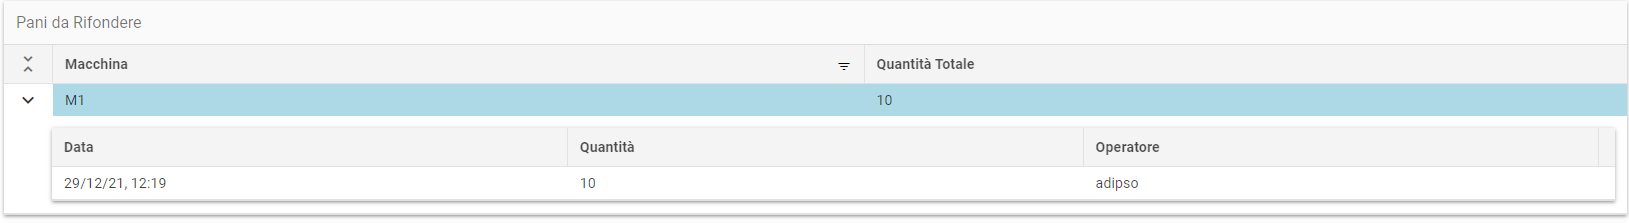
\includegraphics[width = \columnwidth]{PaniDaRifondere}
      \centering
      \caption{\textit{Pani da Rifondere}}
      \label{fig:PaniDaRifondere}
    \end{figure}
    
    \item \textit{Formato e Numero Pacchi}. Questa tabella contiene le informazioni sui pacchi prodotti nell'impianto di colata
    continua come il formato dei pacchi e la quantità. Queste informazioni vengono lette direttamente dal software
    di supervisione. La tabella è visibile nella \textit{Figura \ref{fig:FormatoNumeroPacchi}};

    \begin{figure}[H]
      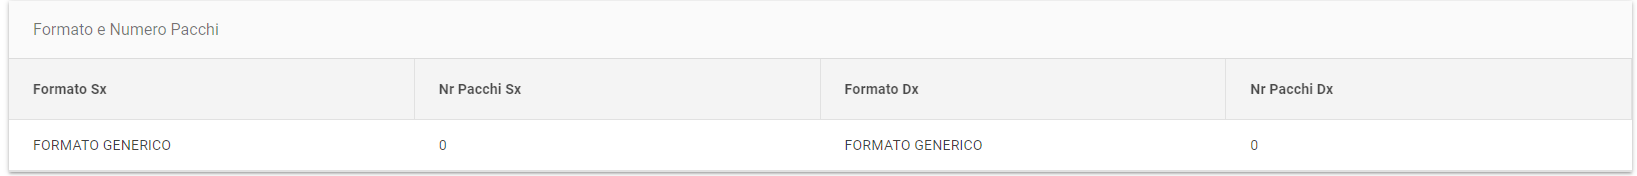
\includegraphics[width = \columnwidth]{FormatoNumeroPacchi}
      \centering
      \caption{\textit{Formato e Numero Pacchi}}
      \label{fig:FormatoNumeroPacchi}
    \end{figure}
    
    \item \textit{Elenco Rallentamenti}. Questa tabella contiene le informazioni relative ai rallentamenti dell'impianto
    che si sono verificati durante la colata selezionata. Le informazioni visualizzate sono la macchina in cui si è verificato
    il rallentamento, la causa, la data di inizio, quella di fine e l'operatore che ha registrato il rallentamento.
    Inoltre è possibile registrare un nuovo rallentamento relativo alla colata selezionata;
    
     \item \textit{Elenco Anomalie}. Questa tabella contiene l'elenco delle anomalie che sono state rilevate nel corso della
    colata selezionata. Le informazioni visualizzate in questa tabella sono la macchina in cui si è verificato il
    rallentamento, la data di rilevazione dell'anomalia, l'operatore che ha inserito l'anomalia, il tipo e la descrizione.
    Inoltre è possibile anche aggiungere una nuova anomalia per la colata selezionata. La tabella è visibile nella
    \textit{Figura \ref{fig:ElencoAnomalie}};
    
    \item \textit{Elenco Fermi}. Questa tabella contiene l'elenco dei fermi rilevati relativi alla colata selezionata 
    e quelli ancora non causalizzati. I fermi sono filtrabili tra quelli causalizzati e quelli non causalizzati,
    che hanno lo sfondo arancione, per differenziarli da quelli causalizzati. Le informazioni visualizzate sono la macchina
    in cui si è verificato il fermo, la data e l'ora di inizio e di fine del fermo, la durata totale, i cinque perchè e
    l'azione correttiva. Inoltre è possibile causalizzare i fermi non causalizzati e aggiungere nuovi fermi manualmente.
    La tabella è visibile nella \textit{Figura \ref{fig:ElencoFermi}};
    
    \item \textit{Elenco Note Colata Corrente}. Questa tabella contiene l'elenco delle note che sono state inserite nel corso
    della colata attuale. Le informazioni visualizzate in questa tabella sono la data di inserimento, l'operatore che ha inserito
    la nota e la nota stessa. Inoltre è possibile aggiungere nuove note. La tabella è visibile nella
    \textit{Figura \ref{fig:ElencoNote}};
    
    \item \textit{Elenco Note Ultime 10 Colate}. Questa tabella contiene l'elenco delle note che sono state inserite durante le
    dieci colate precedenti a quella selezionata. Le informazioni visualizzate sono le stesse visualizzate nella tabella
    contenente le note relative alla colata corrente, con l'aggiunta del numero della colata relativa alla nota;
    
    \item \textit{Passaggio di Consegne}. Questa tabella contiene l'elenco dei passaggi di consegne che sono stati inseriti
    nel corso della colata selezionata. Le informazioni visualizzate in questa tabella sono la data di inserimento, l'operatore
    che ha inserito il passaggio di consegna e la relativa descrizione. Inoltre è possibile aggiungere un nuovo passaggio
    di consegna.
    La tabella è visibile nella \textit{Figura \ref{fig:PassaggioDiConsegne}};

    \begin{figure}[H]
      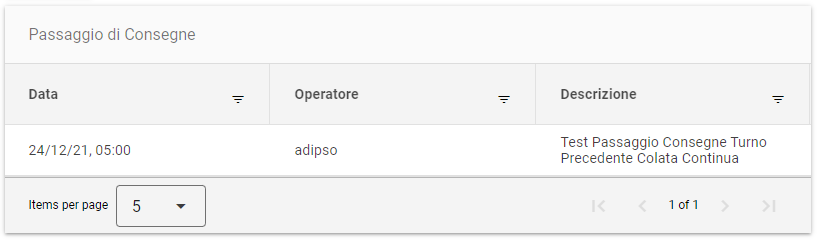
\includegraphics[width = \columnwidth]{PassaggioDiConsegne}
      \centering
      \caption{\textit{Passaggio di Consegne}}
      \label{fig:PassaggioDiConsegne}
    \end{figure}
    
    \item \textit{Passaggio di Consegne Turno Precedente}. Questa tabella contiene l'elenco dei passaggi di consegne che sono
    stati inseriti durante il turno precedente. Le informazioni visualizzate sono le stesse visualizzate nella tabella
    contenente i passaggi di consegna relativi alla colata corrente;
    
    \item \textit{Tempi Componenti}. Questa tabella contiene l'elenco dei componenti che si trovano nel reparto colata continua
    e le ore di funzionamento. Inoltre è anche possibile resettare questo contatore premendo sul pulsante reset. Questi dati
    vengono letti direttamente dal software di supervisione. La tabella è visibile nella \textit{Figura \ref{fig:TempiComponenti}};

    \begin{figure}[H]
      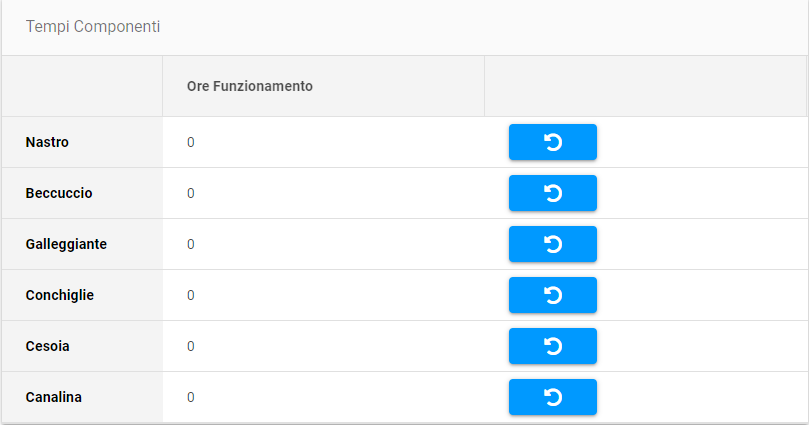
\includegraphics[width = \columnwidth]{TempiComponenti}
      \centering
      \caption{\textit{Tempi Componenti}}
      \label{fig:TempiComponenti}
    \end{figure}

  \end{itemize}

  \section{Rapporti Di Lavoro Magazzino Pani}
  La schermata \textit{Rapporti Di Lavoro Magazzino Pani} permette di visualizzare
  i rapporti di lavoro relativi al Magazzino Pani. Le informazioni visualizzate vengono filtrate in base
  all'anno e alla colata. Di default vengono mostrate le informazioni relative alla colata in corso. Nella schermata vengono
  visualizzate le informazioni sul turno attuale e sulla colata selezionata, oltre che all'operatore di supporto per il turno
  in corso. Inoltre sono visibili le seguenti tabelle che mostrano informazioni relative al rapporto di lavoro:
  \begin{itemize}
    \item \textit{Pesatura Pacchi}. Questa tabella contiene le informazioni sulle tipologie di pacchi e le relative quantità
    che entrano nel magazzino pani. Le informazioni sono relative alle rilevazioni automatiche, lette automaticamente dal
    software di supervisione, alle rilevazioni inserite manualmente e al totale. Inoltre è possibile inserire nuove rilevazioni
    manuali e anche impostare il tempo di pesatura manuale. La tabella è visibile nella 
    \textit{Figura \ref{fig:PesaturaPacchi}};

    \begin{figure}[H]
      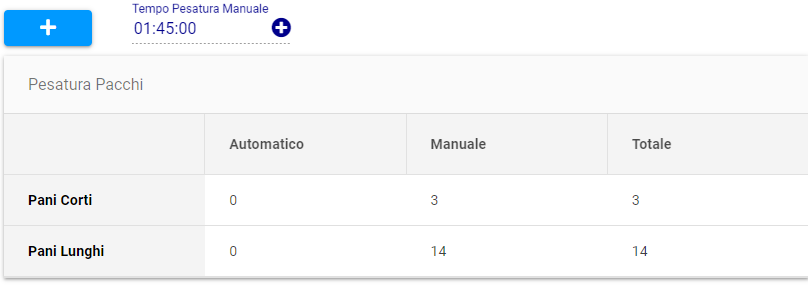
\includegraphics[width = \columnwidth]{PesaturaPacchi}
      \centering
      \caption{\textit{Pesatura Pacchi}}
      \label{fig:PesaturaPacchi}
    \end{figure}

    \item \textit{Interruzoni}. Questa tabella contiene le informazioni sulle interruzioni che si sono verificate durante la
    colata selezionata. Le informazioni visualizzate in questa tabella sono la data di inizio, la data di fine, gli operatori
    che hanno inserito l'inizio e la fine dell'interruzione. Infatti è presente un pulsante che, se non è in corso nessuna interruzione
    consente di inserirne una nuova, altrimenti permette di chiudere l'interruzione già presente. La tabella è
    visibile nella \textit{Figura \ref{fig:Interruzioni}};

    \begin{figure}[H]
      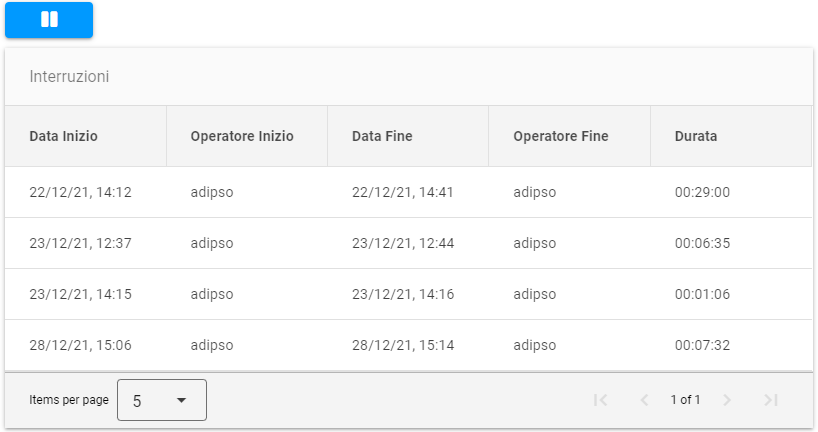
\includegraphics[width = \columnwidth]{Interruzioni}
      \centering
      \caption{\textit{Interruzioni}}
      \label{fig:Interruzioni}
    \end{figure}

    \item \textit{Elenco Fermi}. Questa tabella contiene l'elenco dei fermi rilevati relativi alla colata selezionata 
    e quelli ancora non causalizzati. I fermi sono filtrabili tra quelli causalizzati e quelli non causalizzati,
    che hanno lo sfondo arancione, per differenziarli da quelli causalizzati. Le informazioni visualizzate sono la data e
    l'ora di inizio e di fine del fermo, la durata totale, i cinque perchè e
    l'azione correttiva. Inoltre è possibile causalizzare i fermi non causalizzati e aggiungere nuovi fermi manualmente.
    La tabella è visibile nella \textit{Figura \ref{fig:ElencoFermi}};

    \item \textit{Elenco Note Colata Corrente}. Questa tabella contiene l'elenco delle note che sono state inserite nel corso
    della colata attuale. Le informazioni visualizzate in questa tabella sono la data di inserimento, l'operatore che ha inserito
    la nota e la nota stessa. Inoltre è possibile aggiungere nuove note. La tabella è visibile nella
    \textit{Figura \ref{fig:ElencoNote}};

    \item \textit{Elenco Note Ultime 10 Colate}. Questa tabella contiene l'elenco delle note che sono state inserite durante le
    dieci colate precedenti a quella selezionata. Le informazioni visualizzate sono le stesse visualizzate nella tabella
    contenente le note relative alla colata corrente, con l'aggiunta del numero della colata relativa alla nota;


    \item \textit{Elenco Anomalie}. Questa tabella contiene l'elenco delle anomalie che sono state rilevate nel corso della
    colata selezionata. Le informazioni visualizzate in questa tabella sono la data di rilevazione dell'anomalia,
    l'operatore che ha inserito l'anomalia, il tipo e la descrizione.
    Inoltre è possibile anche aggiungere una nuova anomalia per la colata selezionata.
    La tabella è visibile nella \textit{Figura \ref{fig:ElencoAnomalie}};

    \item \textit{Passaggio di Consenge}. Questa tabella contiene l'elenco dei passaggi di consegna che sono stati inseriti
    nel corso della colata selezionata. Le informazioni visualizzate in questa tabella sono la data di inserimento, l'operatore
    che ha inserito il passaggio di consegna e la relativa descrizione. Inoltre è possibile aggiungere un nuovo passaggio
    di consegna. La tabella è visibile nella \textit{Figura \ref{fig:PassaggioDiConsegne}};

    \item \textit{Passaggio di Consegne Turno Precedente}. Questa tabella contiene l'elenco dei passaggi di consegne che sono
    stati inseriti durante il turno precedente. Le informazioni visualizzate sono le stesse visualizzate nella tabella
    contenente i passaggi di consegne relative alla colata corrente;

  \end{itemize}

  \section{Analisi Chimiche}
  La schermata \textit{Analisi Chimiche}, visibile nella \textit{Figura \ref{fig:AnalisiChimiche}};,
  permette di visualizzzare le informazioni relative alle
  analisi chimiche svolte durante le colate nei forni fusorio e a bacino. Nella pagina relativa alle analisi chimiche sono
  quindi visibili le informazioni sulla colata in corso e l'elenco delle relative analisi chimiche. Di ogni analisi chimica
  è possibile vedere le relative informazioni, come l'id del quantometro, la data di esecuzione dell'analisi, il tipo (o stato) e
  il dettaglio, ovvero l'elenco degli elementi chimici rilevati e la relativa percentuale rilevata, con anche le percentuali
  minime e massime per rispettare lo standard. Inoltre è possibile anche visualizzare l'eventuale proposta di correzione già
  accettata in precedenza, con i relativi materiali correttivi e la quantità da caricare.\\
  In questa schermata è possibile calcolare le correzioni per le analisi chimiche che non rispettano le specifiche. Quando
  viene effettuato il calcolo viene mostrato l'elenco di possibili proposte con l'indicazione del correttivo primario utilizzato
  per effettuare il calcolo. Inoltre, è possibile aggiungere e/o rimuovere altri materiali o modificare la quantità da caricare
  per ogni correttivo. Infine è possibile accettare o rifiutare le proposte di correzione che sono state proposte a seguito del
  calcolo.\\
  L'ultima operazione che è possibile effettuare in questa schermata è quella di assegnare una determinata analisi come
  \textit{Analisi per Cliente} per la relativa colata, ovvero indicare l'analisi chimica definitiva per la colata.

  \begin{figure}[H]
    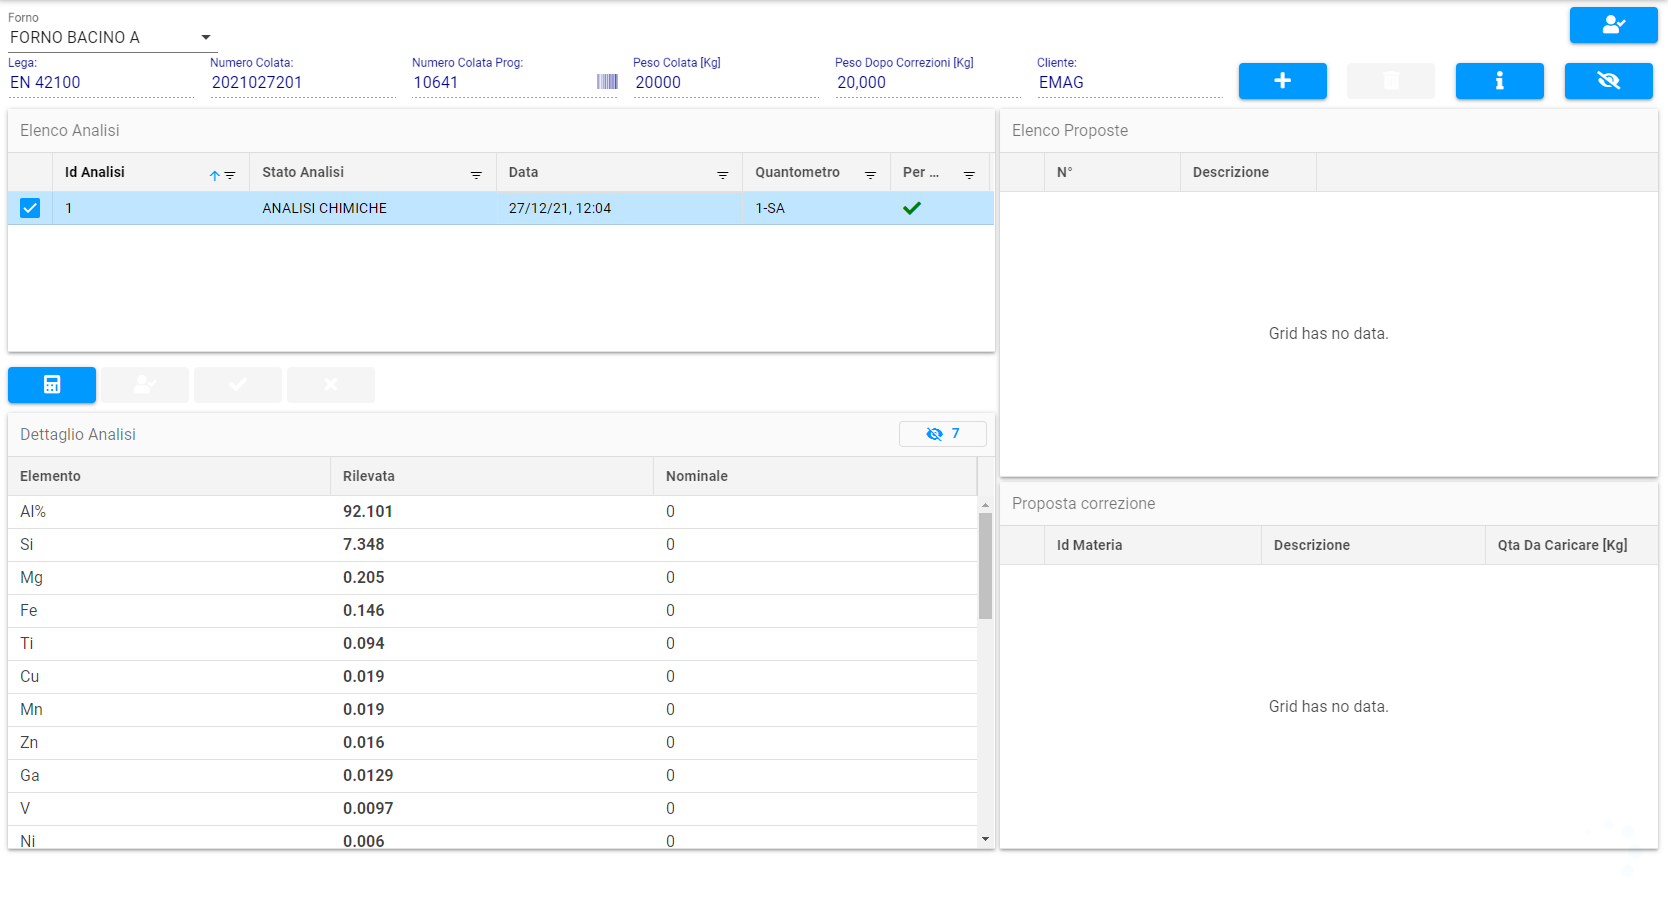
\includegraphics[width = \columnwidth]{AnalisiChimiche}
    \centering
    \caption{\textit{Analisi Chimiche}} 
    \label{fig:AnalisiChimiche}
  \end{figure}

  \section{Materie e Elementi Chimici}
  La schermata \textit{Materie e Elementi Chimici} permette di visualizzare le informazioni
  relative alle anagrafiche delle materie prime e degli elementi chimici. In questa schermata è possibile aggiungere una nuova
  anagrafica o modificarne una esistente. Inoltre, per i materiali correttivi è possibile associare gli elementi chimici
  a un determinato correttivo con l'indicazione della percentuale in cui è contenuto nel correttivo e se il materiale è un
  correttivo primario dell'elemento chimico. 

  \section{Gestione Dizionari}
  La schermata \textit{Gestione Dizionari} permette di visualizzare le informazioni relative
  alle anagrafiche utilizzate nella varie schermate della web application. In questa schermata è possibile aggiungere una nuova
  anagrafica o modificarne una esistente. Le anagrafiche consultabili in questa pagina sono relative ai diversi aspetti
  dell'applicazione, come ad esempio l'elenco dei gruppi utenti, delle pezzature e delle provenienze dei materiali, dei
  tipi di materiale, dei tipi di analisi chimiche, le cause dei rallentamenti e i cinque perchè.
  
  \section{Security}
  La schermata \textit{Security} permette di assegnare ai vari gruppi utente
  le diverse funzionalità della web application e dell'applicativo di supervisione, come la visibilità o meno delle
  diverse schermate e le funzionalità che possono essere eseguite solo da persone autorizzate.